\chapter{Architecture}
Describe the different parts of your program suite in detail.
\\\\
kort inledning till kapitlet. vad har vi gjort i projektet?\\
trattigt namn, borde kanske ändras. ska innehålla typ metod - alltså vad har vi gjort?

\section{Finished work}
Running modules
What does your running code do? what is the output?

\subsection{Naive Bayes}

\subsection{K-Nearest Neighbour (KNN) algorithm}

\subsection{Support Vector Machine (SVM)}

\subsection{The Perceptron algorithm}
The Perceptron algorithm works as follows: 
The output, $w$, from the algorithm is a weight vector with the same size as $y$. If the classification for a $x$ in the training set is equal to $y$, the weight is unchanged.
If $y$ is 1 and the classification -1, then $w$ is increased. If $y$ is -1 and the classification 1, then $w$ is decreased. \citep{perceptron_ai}
\begin{algorithm}[h!]
\label{algorithm:perceptron}
 \SetAlgoLined
 \KwData{data}
 \KwResult{weight vector $w$}
 Initialize weight vector $w$ to all zeros\;
 $N \leftarrow$ number of iterations through training set\;
 \For{1 $\rightarrow$ N}{
   \ForAll{x, y in the training set}{
    $guess \leftarrow classify(x)$ using our current $w$\;
    \If{y is not equal to guess}{
     $w \leftarrow w + f(x, y) - f(x, guess)$\;
     }
   }
 }
 \caption{Perceptron}
\end{algorithm}
The Averaged Perceptron works in the same way except that it returns the average weight vector instead of the final.
This averaged vector is built incrementally by updating it while we build the usual weight vector. The pseudo code almost the same as for the usual perceptron.
\begin{algorithm}[h!]
\label{algorithm:perceptron}
 \SetAlgoLined
 \KwData{data}
 \KwResult{weight vector $w$}
 Initialize weight vector $w$ and the average weight vector $wa$ to all zeros\;
 Initialize the counter $c$ to 0.\;
 $N \leftarrow$ number of iterations through training set\;
 \For{1 $\rightarrow$ N}{
   \ForAll{x, y in the training set}{
    $guess \leftarrow classify(x)$ using our current $w$\;
    \If{y is not equal to guess}{
     $w \leftarrow w + f(x, y) - f(x, guess)$\;
     $average\_weight \leftarrow (N\cdot T - c) / (N\cdot T)$
     $wa \leftarrow wa + average\_weight \cdot (f(x, y) - f(x, guess))$
     }
     Increase the counter c
   }
 }
 \caption{Averaged Perceptron}
\end{algorithm}
In both of the Perceptron algorithms, the algorithm makes a number of iterations. The following plot was made to decide how many iterations that must be done to get a fair result. The algorithms uses input data of 2000 words (unigram) and 10-fold crossvalidaion. As seen in the plot, both the algorithms converge after around 15 iterations for both sentimental classification and text categorization.
\begin{center}
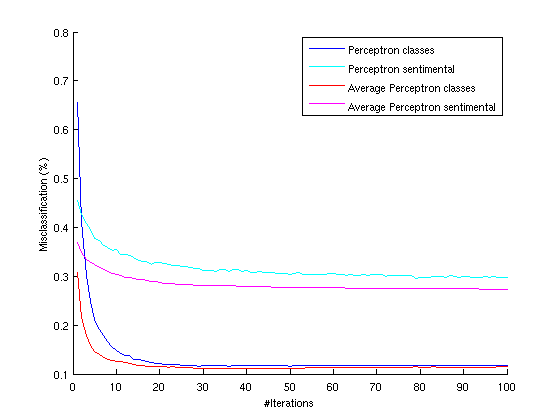
\includegraphics[scale = 0.8]{fig/perceptron_2000words_unigram_10foldcv_classes-high_sentimental-low.png}
\end{center}
Since the Perceptron algorithms are 0/1 classifiers there is some difficulties with classifying the data as classes. This was solved by for all data and all classes classify the data as belonging to this class or not. Finally the new document is classified as the class it belongs to most.

